\documentclass{article}
\usepackage[T2A]{fontenc} 
\usepackage[utf8]{inputenc} 
\usepackage[english,russian]{babel}
\usepackage{graphicx} 
\usepackage{amsmath}
\usepackage{amsfonts} 
\usepackage{titlesec}
\usepackage{listings}
\usepackage{float}
\usepackage{longtable}
\usepackage{titling} 
\usepackage{geometry} 
\usepackage{pgfplots}
\pgfplotsset{compat=1.9}
\usepackage{xcolor}
\definecolor{darkgreen}{RGB}{0,100,0}

\lstset{
  language=Python,
  basicstyle=\ttfamily,
  keywordstyle=\color{darkgreen},
  stringstyle=\color{purple},
  commentstyle=\color{green},
  morecomment=[l][\color{magenta}]{\#},
  frame=single, 
  showspaces=false, 
  showstringspaces=false, 
  numbers=left, 
  numberstyle=\tiny,
}

\titleformat{\section}
  {\normalfont\Large\bfseries}{\thesection}{1em}{}
\titleformat{\subsection}
  {\normalfont\large\bfseries}{\thesubsection}{1em}{}

\setlength{\droptitle}{-6em} 
\title{Отчет по лабораторной работе № 5 и №6\\ Вариант № 3}
\author{Винницкая Дина Сергеевна}
\date{Группа: Б9122-02-03-01сцт}

\geometry{a4paper, margin=2cm}

\begin{document}

\maketitle
\section*{Цель работы}
\begin{enumerate}
    \item Реализовать генерацию сплайна благодаря методу моментов
    \item Сделать таблицу ошибок
    \item Построить график зависимости абсолютной ошибки от количества узлов
    \item Написать вывод о поведении ошибки 
    \item Заключение
\end{enumerate}

\section*{Входные данные:}
\begin{enumerate}
    \item Функция: $f(x) = x^2 + \ln(x) - 4$
    \item Отрезок: $[1.5; 2]$
\end{enumerate}

\section*{Ход работы}
\section*{Реализация сплайна}
Сплайн — это условная функция, которая на каждом узловом отрезке принимает новые коэффициенты для кубического полинома. Для определения этих коэффициентов необходимо получить три массива значений. Для их вычисления используется $\textbf{метод монотонной прогонки}$. \\
$$\textbf{Инициализация функции}$$
\begin{lstlisting}
def function(x):
    return x ** 2 + np.log(x) - 4


def f_derivative_function(x):
    return 2 * x + 1 / x


def s_derivative_function(x):
    return 2 - 1 / (x * x)
\end{lstlisting}
 Задаем исходную функцию, ее первую и вторую производную.
 Первая производная функции \( f(x) \) равна:

\begin{equation}
f'(x) = 2x + \frac{1}{x}
\end{equation}
 Вторая производная функции \( f(x) \) равна:

\begin{equation}
f''(x) = 2 - \frac{1}{x^2}
\end{equation} \\ \\ \\ \\ \\ 


$$\textbf{Инициализация функции}$$
\begin{lstlisting}

def build_spline():
    c_coefficient_matrix = [0] + [h_values[i] / 
    (h_values[i] + h_values[i + 1]) for i in range(0, n - 1)] + [0]
    a_coefficient_matrix = [0] + [h_values[i + 1] / (h_values[i] +
    h_values[i + 1]) for i in range(0, n - 1)] + [0]
    b_coefficient_matrix = [1] + [2] * (n - 1) + [1]

    rhs = [s_derivative_function(interval[0])] + [
        6 / (h_values[i] + h_values[i + 1]) * 
        ((y_values[i + 1] - y_values[i]) / h_values[i + 1] \
        - (y_values[i] - y_values[i -1]) / h_values[i]) for i in
        range(0, n - 1)] + [s_derivative_function(interval[1])]

    alpha = [-c_coefficient_matrix[0] / b_coefficient_matrix[0]]
    betta = [rhs[0] / b_coefficient_matrix[0]]

    moments = [s_derivative_function(interval[1])]

    for i in range(0, n - 1):
        alpha.append(-c_coefficient_matrix[i] / (alpha[i] *
        a_coefficient_matrix[i] + b_coefficient_matrix[i]))
        betta.append((rhs[i] - betta[i] * a_coefficient_matrix[i])
        / (alpha[i] * a_coefficient_matrix[i] + b_coefficient_matrix[i]))

    for i in range(0, n - 1):
        moments.append(alpha[n - i - 1] * moments[i] + betta[n - i - 1])
    moments.append(s_derivative_function(interval[0]));
    moments = moments[::-1]

    a = moments[:-1:]
    b = [(moments[i + 1] - moments[i]) / h_values[i + 1]
    for i in range(0, n)]
    c = [(y_values[i + 1] - y_values[i]) 
    / h_values[i + 1] - h_values[i + 1] / 6 * 
    (2 * moments[i] + moments[i + 1]) for i in range(0, n)]

    return [a, b, c]

\end{lstlisting}

$$\textbf{Описание алгортима}$$

\begin{enumerate}
    \item \textbf{Определение матриц коэффициентов}
    \begin{itemize}
        \item Матрица коэффициентов \( c \) рассчитывается как отношение длины текущего отрезка к сумме длин текущего и следующего отрезков. Начальные и конечные значения этой матрицы равны нулю.
        \item Матрица коэффициентов \( a \) рассчитывается как отношение длины следующего отрезка к сумме длин текущего и следующего отрезков. Начальные и конечные значения этой матрицы также равны нулю.
        \item Матрица коэффициентов \( b \) состоит из единицы в начале и конце, а все промежуточные элементы равны двум.
    \end{itemize}
    
    \item \textbf{Определение правой части уравнения}
    Правая часть уравнения рассчитывается как значения второй производной функции на концах интервала, а для внутренних узлов — как разница отношений разностей значений функции и длин отрезков, умноженная на 6.

    \item \textbf{Инициализация и вычисление массивов \( \alpha \) и \( \beta \)}
    \begin{itemize}
        \item Массив \( \alpha \) инициализируется как отношение начального элемента матрицы \( c \) к начальному элементу матрицы \( b \) с отрицательным знаком.
        \item Массив \( \beta \) инициализируется как отношение начального элемента RHS к начальному элементу матрицы \( b \).
    \end{itemize}

    \item \textbf{Вычисление моментов \( M \)}
    Массив моментов инициализируется значением второй производной функции на правом конце интервала.

    \item \textbf{Обход в прямом порядке для вычисления \( \alpha \) и \( \beta \)}
    Для каждого узла (кроме первого и последнего) массивы \( \alpha \) и \( \beta \) обновляются на основе значений матриц коэффициентов \( a \), \( b \), \( c \) и RHS.

    \item \textbf{Обход в обратном порядке для вычисления моментов \( M \)}
    Для каждого узла (кроме первого и последнего) массив моментов \( M \) обновляется на основе значений массивов \( \alpha \) и \( \beta \).

    \item \textbf{Вычисление коэффициентов \( a \), \( b \) и \( c \)}
    \begin{itemize}
        \item Коэффициенты \( a \) равны всем элементам массива моментов \( M \), кроме последнего.
        \item Коэффициенты \( b \) рассчитываются как разница соседних элементов массива моментов \( M \), деленная на длину соответствующих отрезков.
        \item Коэффициенты \( c \) рассчитываются как разница значений функции в соседних узлах, деленная на длину соответствующих отрезков, с корректировкой на основе длин отрезков и значений моментов.
    \end{itemize}

    \item \textbf{Возврат коэффициентов}
    Функция возвращает массивы коэффициентов \( a \), \( b \) и \( c \), которые используются для вычисления непосредственного сплайна.
    
\end{enumerate}
$$\textbf{Реализация сплайна}$$
\begin{lstlisting}
def evaluate_spline(x, i):
    return y_values[i] + spline_coefficients[2][i] * (x - x_values[i]) 
    + spline_coefficients[0][i] * (
            x - x_values[i]) ** 2 / 2 + spline_coefficients[1][i] 
            * (x - x_values[i]) ** 3 / 6


x_values = np.linspace(*interval, 20)
n = len(x_values) - 1
h_values = [abs(x_values[_] - x_values[_ - 1]) for _ in range(0, n + 1)]
y_values = [function(_) for _ in x_values]

spline_coefficients = build_spline()

for i in range(n):
    xl = np.linspace(x_values[i], x_values[i + 1], 10)
    yl = evaluate_spline(xl, i)

    plt.plot(xl, yl)
\end{lstlisting}

$$\textbf{Алгоритм}$$
\begin{enumerate}
    \item \textbf{Создание сетки значений \( x \)}:
    Генерируется массив из 20 равномерно распределенных значений \( x \) на заданном интервале.
    
    \item \textbf{Вычисление длин отрезков \( h \)}:
    Вычисляются длины каждого отрезка между узлами.
    
    \item \textbf{Вычисление значений функции \( y \)}:
    Вычисляются значения функции \( f(x) \) в каждом узле.
    
    \item \textbf{Построение коэффициентов сплайна}:
    Вызывается функция \texttt{build\_spline} для вычисления коэффициентов сплайна.
    
    \item \textbf{Визуализация сплайна}:
    Для каждого интервала вычисляются значения сплайна и строится график на данном интервале.
\end{enumerate}
$$\textbf{График}$$
\begin{figure}[H]
    \centering
    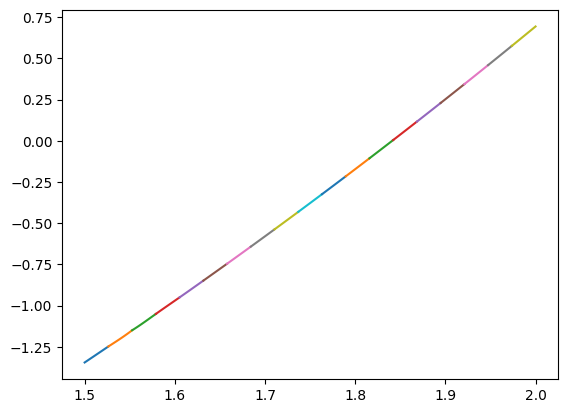
\includegraphics[width=0.7\textwidth]{lab_5_6_1.png}
    \caption{График сплайна}
    \label{fig:my_label}
\end{figure}
\section*{Ошибки}
$$\textbf{Реализация}$$

\begin{lstlisting}
def norm(lst):
    return max(list(map(np.fabs, lst)))
ns = [3, 5, 10, 20, 30, 40, 55, 70, 85, 100]
max_deviations = []
relative_deviations = []

for num_intervals in ns:

    spline_y_values = []
    x_values = np.linspace(*interval, num_intervals)
    n = num_intervals - 1
    h_values = [abs(x_values[_] - x_values[_ - 1]) for _ in 
    range(0, n + 1)]
    y_values = [function(_) for _ in x_values]
    
    spline_coefficients = build_spline()
    
    for i in range(n):
        xl = np.linspace(x_values[i], x_values[i + 1], 10)
        yl = evaluate_spline(xl, i)

        spline_y_values += [*yl]
    original_y_values = function(np.linspace(*interval, n * 10))

    spline_norm = norm(np.array(spline_y_values) - original_y_values)
    function_norm = norm(original_y_values)
    max_deviations.append(spline_norm)
    relative_deviations.append(spline_norm / function_norm * 100)
    print(num_intervals, spline_norm, spline_norm
    / function_norm * 100, sep='\t')

\end{lstlisting}

$$\textbf{Алгоритм}$$

\textbf{\texttt{norm(lst)} возвращает максимальное абсолютное значение списка.}

\textbf{Задаются числа интервалов (\texttt{ns}) и списки для отклонений.}

\textbf{Цикл по числу интервалов}
    \begin{itemize}
        \item Для каждого значения \texttt{num\_intervals}:
        \begin{itemize}
            \item Генерация сетки \( x \), вычисление длин отрезков \( h \) и значений функции \( y \).
            \item Построение коэффициентов сплайна.
            \item Вычисление значений сплайна и добавление их в список.
            \item Вычисление значений оригинальной функции на плотной сетке.
            \item Вычисление максимального и относительного отклонений.
            \item Добавление отклонений в списки.
        \end{itemize}
    \end{itemize}

$$\textbf{Таблица ошибок}$$
    \begin{table}[h!]
    \centering
    \begin{tabular}{|c|c|c|}
        \hline
        \textbf{n} & \textbf{Абсолютное отклонение} & \textbf{Относительное отклонение} \\
        \hline
        3   & 0.05371643350201083   & 3.9951684278292565  \\
        \hline
        5   & 0.04343490397994143   & 3.230478007069501   \\
        \hline
        10  & 0.022010032911421007  & 1.6369997568788763  \\
        \hline
        20  & 0.011168471008359937  & 0.8306568372238579  \\
        \hline
        30  & 0.00746909969040388   & 0.555515497250833   \\
        \hline
        40  & 0.0056090498036676095 & 0.417173986148873   \\
        \hline
        55  & 0.004083074671390463  & 0.3036793389307547  \\
        \hline
        70  & 0.00320965733824341   & 0.23871878354359727 \\
        \hline
        85  & 0.002644010127457186  & 0.1966486807744287  \\
        \hline
        100 & 0.002247842609951256  & 0.16718365759838455 \\
        \hline
    \end{tabular}
    \caption{Таблица абсолютных и относительных отклонений}
    \label{table:deviations}
    \end{table}

$$\textbf{График зависимости абсолютной ошибки от количества узлов}$$
\begin{figure}[H]
    \centering
    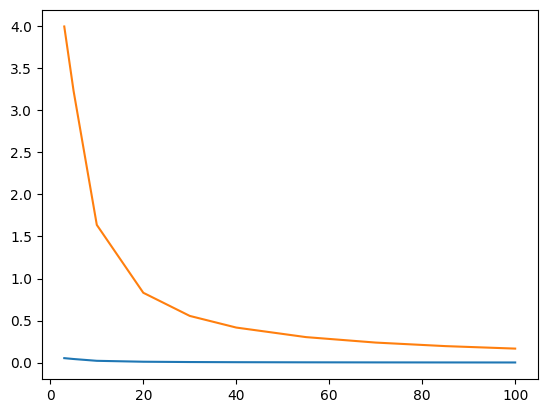
\includegraphics[width=0.7\textwidth]{lab_5_6_2.png}
    \caption{График сплайна}
    \label{fig:my_label}
\end{figure}

\section*{Вывод о поведении ошибок}

На основе приведенных данных можно сделать следующие выводы:

\begin{itemize}
    \item \textbf{Уменьшение абсолютного отклонения (\( \Delta \))}: С увеличением количества интервалов \( n \), абсолютное отклонение (\( \Delta \)) последовательно уменьшается. Это свидетельствует о том, что аппроксимация сплайном становится точнее при увеличении числа интервалов.
    \item \textbf{Уменьшение относительного отклонения (\( \delta \))}: Аналогично, относительное отклонение (\( \delta \)) также уменьшается с увеличением числа интервалов. Это показывает, что относительная погрешность аппроксимации снижается, делая аппроксимацию более точной по сравнению с исходной функцией.
    \item \textbf{Скорость уменьшения отклонений}: Как видно из данных, наиболее значительное снижение отклонений наблюдается при малых значениях \( n \). При больших значениях \( n \) уменьшение отклонений становится менее выраженным. Это может свидетельствовать о том, что дальнейшее увеличение числа интервалов приводит к менее значимому улучшению точности аппроксимации.
\end{itemize}

В целом, результаты подтверждают, что увеличение числа интервалов \( n \) улучшает точность аппроксимации сплайном как в абсолютном, так и в относительном выражении.

\section*{Заключение}


В данной лабораторной работе была проведена аппроксимация функции с использованием кубических сплайнов. Основные этапы включали:
\begin{enumerate}
    \item Разбиение заданного интервала на различные числа интервалов.
    \item Вычисление значений функции и её производных в узловых точках.
    \item Построение коэффициентов кубических сплайнов.
    \item Оценка погрешности аппроксимации путем вычисления максимальных и относительных отклонений.
\end{enumerate}


На основе проведенных экспериментов и анализа полученных данных были сделаны следующие выводы:
\begin{enumerate}
    \item \textbf{Точность аппроксимации}: С увеличением числа интервалов \( n \) максимальное отклонение (\( \Delta \)) и относительное отклонение (\( \delta \)) последовательно уменьшаются. Это свидетельствует о повышении точности аппроксимации кубическим сплайном при увеличении числа интервалов.
    \item \textbf{Скорость сходимости}: Наиболее значительное снижение отклонений наблюдается при малых значениях \( n \). При больших значениях \( n \) уменьшение отклонений становится менее выраженным, что указывает на уменьшение эффекта от дальнейшего увеличения числа интервалов.
    \item \textbf{Практическое применение}: Аппроксимация кубическими сплайнами показала свою эффективность для точного представления функций. Метод может быть полезен в различных прикладных задачах, требующих высокой точности аппроксимации.
\end{enumerate}



\end{document}

